\section{Moment pędu}

\subsection{Momentu pędu w mechanice klasycznej}
W mechanice klasycznej moment pędu (inaczej moment kątowy) cząstki względem punktu odniesienia definiujemy jako iloczyn wektorowy położenia $\vec{r}$ i pędu $\vec{p}$
$$
\vec{L} = \vec{r} \times \vec{p}.
$$
\begin{figure}[H]
\centering
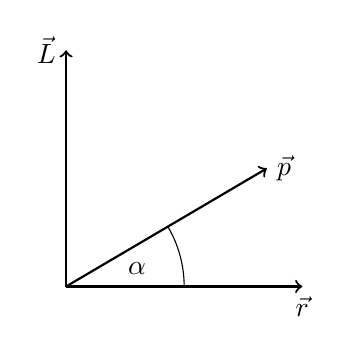
\begin{tikzpicture}[scale=1.5]
\begin{scope}
  \draw[->, thick] (0,0) -- (2,0) node[below] {$\vec{r}$};
  \draw[->, thick] (0,0) -- (0,2) node[left] {$\vec{L}$};
  \draw[->, thick] (0,0) -- (1.7,1) node[right] {$\vec{p}$};
  \draw (1,0) arc (0:30:1);
  \node at (0.6,0.15) {$\alpha$};
\end{scope}
\end{tikzpicture}
\caption{Moment pędu jako iloczyn wektorowy $\vec{r}$ i $\vec{p}$.}
\end{figure}

Wartość bezwzględna momentu pędu wynosi
$$
|\vec{L}| = |\vec{r}| \cdot |\vec{p}| \cdot \sin \alpha,
$$
gdzie $\alpha$ to kąt między wektorami $\vec{r}$ i $\vec{p}$. Moment pędu jest więc wielkością wektorową, prostopadłą do płaszczyzny rozpiętej przez $\vec{r}$ i $\vec{p}$.
\begin{figure}[H]
\centering
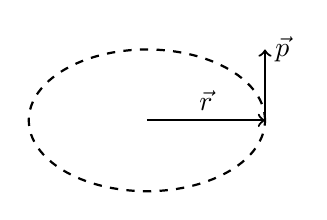
\begin{tikzpicture}[scale=1.5]
\begin{scope}
  \draw[dashed, thick] (0,0) ellipse (1 and 0.6);
  \draw[->, thick] (0,0) -- (1,0) node[midway, above] {$\vec{r}$};
  \draw[->, thick] (1,0) -- (1,0.6) node[right] {$\vec{p}$};
\end{scope}
\end{tikzpicture}
\caption{Moment pędu jako wektor prostopadły do płaszczyzny rozpiętej przez $\vec{r}$ i $\vec{p}$.}
\end{figure}

\subsection{Zasada zachowania momentu pędu}
W układach \textbf{stacjonarnych}, czyli takich, w których nie zmieniają się parametry układu w czasie, zachodzi zasada zachowania momentu pędu
$$
\frac{d\vec{L}}{dt} = 0 \quad \Rightarrow \quad \vec{L} = \text{const.}
$$
Oznacza to, że moment pędu nie ulega zmianie w czasie, jeśli na układ nie działa moment sił zewnętrznych (np. brak momentu zewnętrznego lub centralna symetria pola).

Zachowanie całkowitego momentu pędu wynika z symetrii układu, a w szczególności z~\textbf{symetrii osiowej}. W języku mechaniki klasycznej mówi się wówczas, że jest to \textbf{całka ruchu}.

\subsection{Moment pędu w mechanice kwantowej}
W mechanice kwantowej moment pędu staje się \textbf{operatorem}. Składowe klasycznego momentu pędu można zapisać w postaci
$$
\begin{aligned}
L_x &= y p_z - z p_y, \\
L_y &= z p_x - x p_z, \\
L_z &= x p_y - y p_x.
\end{aligned}
$$

Po przejściu do przestrzeni operatorów (czyli do formalizmu mechaniki kwantowej), każdej z wielkości przypisujemy odpowiedni operator. Operatory składowych momentu pędu przyjmują postać
$$
\begin{aligned}
\hat{L}_x &= -i\hbar \left( y \frac{\partial}{\partial z} - z \frac{\partial}{\partial y} \right), \\
\hat{L}_y &= -i\hbar \left( z \frac{\partial}{\partial x} - x \frac{\partial}{\partial z} \right), \\
\hat{L}_z &= -i\hbar \left( x \frac{\partial}{\partial y} - y \frac{\partial}{\partial x} \right),
\end{aligned}
$$
gdzie $\hbar$ to zredukowana stała Plancka.

Operator momentu pędu jako wielkość wektorowa zapisuje się ogólnie w postaci
$$
\vec{\hat{L}} = -i\hbar\, \vec{r} \times \vec{\nabla},
$$
gdzie $\vec{r} = (x, y, z)$ jest operatorem położenia, a $\vec{\nabla} = \left( \frac{\partial}{\partial x}, \frac{\partial}{\partial y}, \frac{\partial}{\partial z} \right)$ jest operatorem gradientu.

\subsection{Komutatory operatorów momentu pędu}
$$
\begin{aligned}
[L_x, L_y] &= [y p_z - z p_y, z p_x - x p_z] \\
&= [y p_z, z p_x] - [z p_y, z p_x] - [y p_z, x p_z] + [z p_y, x p_z]
\end{aligned}
$$

$$
[yp_z, zp_x] = yp_z zp_x - zp_x yp_z = y p_x [p_z, z] = -i\hbar y p_x
$$

Poniżej przedstawione są komutatory
$$
\begin{aligned}
  [\hat{L}_x, \hat{L}_y] &= i\hbar(xp_y - yp_x) = i \hbar \hat{L}_z, \\
  [\hat{L}_y, \hat{L}_z] &= i \hbar \hat{L}_x, \\
  [\hat{L}_z, \hat{L}_x] &= i \hbar \hat{L}_y.
\end{aligned}
$$
Z powyższych relacji wynika, że operatory składowych momentu pędu nie komutują ze sobą
$$
[\hat{L}_x, \hat{L}_y] \neq 0,
$$
co oznacza, że nie można jednocześnie znać dokładnych wartości wszystkich trzech składowych momentu pędu.

Gdyby nie operatory to poniższa relacja byłaby sprzeczna
$$
\hat{\vec{L}} \times \hat{\vec{L}} = i\hbar \hat{\vec{L}}.
$$

\subsection{Operator $\hat{L}^2$}
Kwadrat całkowitego momentu pędu zdefiniowany jest jako
$$
\hat{L}^2 = \hat{L}_x^2 + \hat{L}_y^2 + \hat{L}_z^2.
$$
Działa on jako operator skalarowy. Co istotne, komutuje ze wszystkimi składowymi momentu pędu
$$
[\hat{L}^2, \hat{L}_x] = [\hat{L}^2, \hat{L}_y] = [\hat{L}^2, \hat{L}_z] = 0.
$$
Zatem można jednocześnie mierzyć $\hat{L}^2$ i jedną wybraną składową, np. $\hat{L}_z$.

\subsection{Wybór układu współrzędnych -- baza sferyczna}
W przypadku momentu pędu wygodnie jest przejść do współrzędnych sferycznych. Przejście z kartezjańskich do sferycznych opisuje się wzorami:
$$
\begin{aligned}
x &= r \sin \theta \cos \varphi, \\
y &= r \sin \theta \sin \varphi, \\
z &= r \cos \theta.
\end{aligned}
$$
W tej bazie wyrażenia dla operatorów $\hat{L}_z$ i $\hat{L}^2$ przyjmują szczególnie prostą postać, co umożliwia rozwiązywanie równań własnych i wyznaczanie funkcji własnych momentu pędu (sferyczne funkcje harmoniczne).


\subsection{Operator momentu pędu w współrzędnych sferycznych}
W układzie sferycznym wyrażenia dla operatorów momentu pędu upraszczają się i zależą tylko od kątów $\theta$ i $\varphi$. Składowe operatora momentu pędu mają następującą postać:
$$
\begin{aligned}
\hat{L}_x &= -i\hbar \left( \sin\varphi \frac{\partial}{\partial\theta} + \cot\theta \cos\varphi \frac{\partial}{\partial\varphi} \right) \\
\hat{L}_y &= -i\hbar \left( -\cos\varphi \frac{\partial}{\partial\theta} + \cot\theta \sin\varphi \frac{\partial}{\partial\varphi} \right) \\
\hat{L}_z &= -i\hbar \frac{\partial}{\partial\varphi}
\end{aligned}
$$

Kwadrat momentu pędu $\hat{L}^2$ w układzie sferycznym wyraża się jako
$$
\hat{L}^2 = -\hbar^2 \left[ \frac{1}{\sin\theta} \frac{\partial}{\partial\theta} \left( \sin\theta \frac{\partial}{\partial\theta} \right) + \frac{1}{\sin^2\theta} \frac{\partial^2}{\partial\varphi^2} \right]
$$

Jest to tzw. \textbf{operator Laplace’a-Beltramiego} na sferze jednostkowej, który jest kluczowy w~opisie funkcji własnych momentu pędu, czyli sferycznych funkcji harmonicznych.

Nie ma zależności między funkcjami własnymi różnych składowych. Z operatorów $\hat{L}_x, \hat{L}_y, \hat{L}_z$ tylko jedna składowa może być jednocześnie diagonalizowana razem z $\hat{L}^2$. Zatem
$$
[\hat{L}_i, f(\theta, \varphi)] \ne 0 \quad \text{dla } i = x, y.
$$

$$
V_n = \vec{n} \cdot \vec{V} = n_x V_x + n_y V_y + n_z V_z \quad ; \quad \vec{w} = \vec{u} \times \vec{v}, \; \norm{\vec{w}} = \norm{\vec{u}} = \norm{\vec{v}} = 1
$$
Z tego wynika analogiczna algebra komutatorów
$$
[L_u, L_v] = i\hbar L_w \quad ; \quad [L_v, L_w] = i\hbar L_u \quad ; \quad [L_w, L_u] = i\hbar L_v
$$

\subsection{Układ złożony z wielu cząstek}
Załóżmy, że mamy $N$ cząstek. Wtedy całkowity moment pędu układu to suma momentów pędu poszczególnych cząstek
$$
\hat{\vec{L}} = \sum_{i=1}^N \vec{r}_i \times \hat{\vec{p}}_i = \sum_{i=1}^N \hat{\vec{L}}_i.
$$

Każdy z operatorów zachowuje tę samą strukturę komutatorów jak w przypadku jednej cząstki
$$
[\hat{L}_x, \hat{L}_y] = i\hbar \hat{L}_z, \quad \text{itd.}
$$

